%
% Paper on anomalies that can occur when applying the BLUE method
% to combined two measurements.
%
% Michael Schmitt      Northwestern University   Sep 2016
%
\documentclass[11pt]{article}
\textwidth=6.5in
\textheight=8.5in
\hoffset=-0.5in
\voffset=-1in
\usepackage{graphicx}
\usepackage{amsmath,amsthm,amssymb}

\usepackage{color}
\definecolor{darkred}{rgb}{0.6,0.0,0.}
\newcommand{\darkred}{\color{darkred}}
\definecolor{navy}{rgb}{0.,0.,0.502}
\newcommand{\navy}{\color{navy}}
\definecolor{purple}{rgb}{0.4,0.,0.4}
\newcommand{\purple}{\color{purple}}

\newcommand{\chisq} {\chi^2}
\newcommand{\chisqmin} {\chi^2_{\mathrm{min}}}
\newcommand{\xtrue} {x_{\mathrm{true}}}
\newcommand{\xa}   {x_1}
\newcommand{\xb}   {x_2}
\newcommand{\uast} {\sigma_{1,\mathrm{stat}}}
\newcommand{\ubst} {\sigma_{2,\mathrm{stat}}}
\newcommand{\uasy} {\sigma_{1,\mathrm{sys}}}
\newcommand{\ubsy} {\sigma_{2,\mathrm{sys}}}
\newcommand{\uastq} {\sigma^2_{1,\mathrm{stat}}}
\newcommand{\ubstq} {\sigma^2_{2,\mathrm{stat}}}
\newcommand{\uasyq} {\sigma^2_{1,\mathrm{sys}}}
\newcommand{\ubsyq} {\sigma^2_{2,\mathrm{sys}}}

\newcommand{\ua} {\sigma_{1}}
\newcommand{\ub} {\sigma_{2}}
\newcommand{\uc} {\sigma_{c}}
\newcommand{\uaq} {\sigma^2_{1}}
\newcommand{\ubq} {\sigma^2_{2}}
\newcommand{\ucq} {\sigma^2_{c}}

\newcommand{\ca}{c_1}
\newcommand{\cb}{c_2}




\begin{document}
%===============================================
\begin{center}
{\large\bf  BLUE Anomalies}  \\
Michael Schmitt, Northwestern University\\
\today
\end{center}




\section{Overview}
\par
The BLUE method~\cite{Lyons} is popular for combining measurements of a given quantity.
Under certain conditions, however, the result can be anomalous (i.e., counter-intuitive):
the combined value turn out to be lower than the input values or higher than
the input values.   We try to show how this comes about.
\par
{\bf (Out of context.)}
Systematic uncertainties can often be classified as ``multiplicative'' or ``additive.''
Consider the measurement of a cross section, for example:
$$
  \sigma = \frac{ N - B }{\epsilon\,A\,L}
$$
where $N$ is the number of selected events, $B$ is the estimated number of 
selected background events, $\epsilon$ is the efficiency of the selection,
$A$ is the geometric and kinematic acceptance, and $L$ is the integrated
luminosity.   Systematic uncertainties for~$B$ are additive, while systematic
uncertainties for $\epsilon$, $A$, and $L$ are multiplicative.
\par
If a multiplicative uncertainty such as the luminosity uncertainty is common to two
measurements, then it is common to the combined measurement.  Therefore, it
should not be included in the covariance matrix when making the combination.
{\bf Expand this.}

\par
{\purple Make the distinction between uncertainties that can be reduced by
repeating the measurement in exactly the same way, and those that cannot.
The former are statistical, and the latter are systematic.}




\section{Derivation}
\par
We consider the simple example of combining two measurements of
the {\em same} quantity:
$$
 \xa  \pm \uast \pm \uasy
 \qquad {\mathrm{and}} \qquad
 \xb \pm \ubst \pm \ubsy 
$$
where the measured values are $\xa$ and $\xb$,
with statistical uncertainties $\uast$ and $\ubst$ and
systematic uncertainties $\uasy$ and $\ubsy$.
The BLUE method is equivalent to finding the combined value~$c$
using a least-squares method.
\par
One must construct a covariance matrix by summing a matrix
for the statistical uncertainties and another one for the systematic uncertainties.
We take the measurements to be statistically independent, but
with fully correlated systematic uncertainties.  So
\begin{eqnarray}
 {\mathbf{V}} &=&  {\mathbf{V}}_{\mathrm{stat}} + {\mathbf{V}}_{\mathrm{stat}} \cr
 \left( \begin{array}{cc}
   \uaq & \rho\ua\ub \cr \rho\ua\ub & \ubq \cr
          \end{array} \right) &=&
 \left( \begin{array}{cc}
   \uastq & 0 \cr 0 & \ubstq \cr
          \end{array} \right) +
 \left( \begin{array}{cc}
   \uasyq & \pm\uasy\ubsy \cr \pm\uasy\ubsy & \ubsyq \cr
          \end{array} \right) 
\end{eqnarray}
where $\uaq = \uastq + \uasyq$, $\ubq = \ubstq + \ubsyq$, and
$$
 \rho = \frac{ \pm \uasy \ubsy }{ \ua\ub }
  = \frac{ \pm \uasy \ubsy }
 { \sqrt{ \uastq + \uasyq } \, \sqrt{ \ubstq + \ubsyq } } .
$$
The correlation coefficient $\rho$ is close to zero if the statistical uncertainties
dominate, and can be close to $\pm 1$ if the correlated systematic uncertainties dominate.
\par
This covariance matrix is the central element for the $\chi^2$ calculation:
\begin{equation} \label{eq:chisqdef}
 \chi^2 =
 \left( \begin{array}{cc} c-\xa & c-\xb \cr \end{array} \right)
  \left( \begin{array}{cc}
   \uaq & \rho\ua\ub \cr \rho\ua\ub & \ubq \cr
          \end{array} \right)^{-1}
 \left( \begin{array}{c} c - \xa \cr c - \xb \end{array} \right) .
\end{equation}
where $c$ is the single free parameter and represents the combined
value for the measured quantity.  The inverse of the covariance matrix is
$$
{\mathbf{V}}^{-1} = \frac{1}{1 - \rho^2} \,
  \left( \begin{array}{cc}
   \frac{1}{\uaq} & -\frac{\rho}{\ua\ub} \cr -\frac{\rho}{\ua\ub} & \frac{1}{\ubq} \cr
          \end{array} \right) .
$$
A little bit of algebra leads to
$$
 \chi^2 = \frac{1}{1 - \rho^2} \left[
  \frac{(c-\xa)^2}{\uaq} - \frac{2\rho}{\ua\ub} (c-\xa)(c-\xb) + \frac{(c-\xb)^2}{\ubq}
  \right] .
$$
If $\rho = 0$, meaning that the two measurements are completely independent,
then the expression for~$\chi^2$ is transparent:
$$
 \chi^2 =   \frac{(c-\xa)^2}{\uaq}  + \frac{(c-\xb)^2}{\ubq}  .
$$
The minimization of $\chi^2$ with respect to~$c$ leads to
\begin{equation}
\label{eq:csol}
 c = \frac{
 \frac{\xa}{\uaq} - 2\rho\frac{(\xa+\xb)/2}{\ua\ub} + \frac{\xb}{\ubq} 
 }{
  \frac{1}{\uaq} - \frac{2\rho}{\ua\ub} + \frac{1}{\ubq} 
 } =
 \frac{ \xa (\ubq - \rho \ua\ub ) + \xb (\uaq - \rho \ua\ub ) }
      { \ubq - 2 \rho \ua\ub + \uaq } .
\end{equation}
Again, with $\rho = 0$, the result is familiar:
$$
 c = \frac{
 \frac{\xa}{\uaq} + \frac{\xb}{\ubq} 
 }{
  \frac{1}{\uaq} + \frac{1}{\ubq} 
 } 
$$
which is just the weighted average of $\xa$ and $\xb$.
\par
In the special case that $\ua = \ub$, $c = (\xa + \xb)/2$ independently of~$\rho$.
\par
The uncertainty of $c$ is related to the curvature of~$\chi^2$ at its minimum:
the greater the curvature, the tighter the constraint on~$c$.  In fact, if
$\uc$ is the uncertainty for~$c$, then
$$
 \frac{1}{\ucq} = \frac{1}{2} 
 \left. \frac{\partial^2 \chi^2}{\partial c^2} \right|_{\mathrm{min}}
 = \frac{1}{1 - \rho^2} \left(
  \frac{1}{\uaq} - \frac{2\rho}{\ua\ub} + \frac{1}{\ubq}
  \right) 
$$
or
$$
 \uc = \frac{ \sqrt{1 - \rho^2}\, \ua \ub}{\sqrt{ \uaq - 2\rho\ua\ub + \ubq }} 
 = \left( \frac{\ua \ub}{\ua + \ub} \right)
 \frac{ \sqrt{1 - \rho^2} } {\sqrt{ 1 - 2 (1 + \rho ) \frac{\ua\ub}{(\ua+\ub)^2} }  } 
$$
where it may help to recall that $0 \le \ua\ub/(\ua+\ub)^2 \le 1/4$.
When $\ua = \ub$ then
$$
 \uc = \frac{\ua}{\sqrt{2}} \sqrt{ \frac{1 + \rho}{1 - \rho} }
$$
which gives $\uc \rightarrow 0$ when $\rho \rightarrow -1$, i.e.,
if two measurements are perfectly anti-correlated, then their combined
value has no uncertainty -- basically, the fluctuations cancel each
other out.   When $\rho \rightarrow 1$, however, $\uc \rightarrow \infty$,
showing that two measurements that are perfectly correlated must give
the same value, which implies $\ua = \ub = 0$ (i.e., there are no
fluctuations).   These two extremes are obviously artificial and perhaps
even paradoxical, indicating that values of~$\rho$ close to $\pm 1$ have
to be handled with extreme care.





\subsection{Algebraic approach}
\par
The question is: what happens if $\rho$ is definitely not zero?
\par
We first simply carry out the algebraic solution.
Without loss of generality, we take $\xb =  \xa + \Delta$ with $\Delta > 0$.
Furthermore, we can set $\xa = 0$.  Then,
$$
 c = \left(
 \frac{ \frac{1}{\ubq}  - \frac{\rho}{\ua\ub} }
        {   \frac{1}{\uaq} - \frac{2\rho}{\ua\ub} + \frac{1}{\ubq}  }
        \right) \, \Delta .
$$
The two anomalous cases would be  $c < 0$ or $c > \Delta$.
Since we have chosen $\Delta > 0$, we can have $c < 0$ only if
$$
 \frac{1}{\ubq} - \frac{\rho}{\ua\ub} < 0
 \qquad {\mathrm{or}} \qquad
 \rho > \frac{\ua}{\ub}
$$
which is possible if $\ua < \ub$.
We can only have $c > \Delta$ if
$$
 \frac{1}{\ubq} - \frac{\rho}{\ua\ub} > \frac{1}{\ubq} - \frac{2}{\ua\ub} + \frac{1}{\uaq}
 \qquad {\mathrm{or}} \qquad
 \rho >  \frac{\ub}{\ua}
$$
which is possible if  $\ub < \ua$.
\par
What happens at the special values for $\rho$?
For example, suppose $\ua < \ub$ and $\rho = \ua/\ub$.  
The $\chi^2$ function collapses into a transparent form,
$$
 \chi^2 = \frac{c^2}{\uaq} + \frac{\Delta^2}{\ubq-\uaq}
  = \frac{(c-\xa)^2}{\uaq} + \frac{(\xb-\xa)^2}{\ubq-\uaq} 
$$
and by Eq~(\ref{eq:csol}), $c = \xa$, and of course $\uc = \ua$.
Apparently the measurement $\xb$ is ignored.  
The covariance matrix has the special form
$$
 {\mathbf{V}} =  
 \left( \begin{array}{cc}
   \uaq & \uaq \cr \uaq & \ubq \cr
          \end{array} \right) 
$$
where the off-diagonal elements are the same as the
smaller of the two variances.  In the other case with
$\rho = \ub/\ua \le 1$, $c = \xb$ and $\uc = \ub$.
It is surprising that in these specific special cases,
the best result is to take the measurement with the
smaller uncertainty and to ignore the other.
\par
After some algebraic manipulations, we can show that
\begin{equation}
\label{eq:chisqmin}
 \chisqmin = \frac{\Delta^2}{\uaq - 2\rho\ua\ub + \ubq} 
\end{equation}
where $\Delta = \xb - \xa > 0$.  There is only one degree of
freedom, and although the probability distribution for $\chi^2$
peaks at zero and is highly skewed, we will have $E[\chi^2] = 1$
for the expectation value.  Taking $\chi^2 = 1$, 
$(\xb-\xa)^2 = \uaq - 2\rho\ua\ub + \ubq$.    In the extreme
case of completely anticorrelated measurements, 
$$
  \xb - \xa = \ua + \ub ,
$$
which suggests that there is relatively more room for
differences $\xb - \xa$.   If, however, the two measurements
are completely correlated, then
$$
  \xb - \xa = | \ub - \ua |
$$
which means that only rather close values of the measurements
lead to a good value of $\chi^2$, and in the case $\ub \rightarrow \ua$,
a finite difference $\Delta > 0$ always leads to a bad $\chi^2$.
Although these two extreme cases are artificial (note, for example,
that the covariance matrix is singular when $\rho = \pm 1$), they are intuitive.
For anticorrelated measurements, one value fluctuating upward is paired
with another that fluctuates downward, hence their difference should be
relatively large.  For strongly correlated measurements, however, one
value fluctuating upward should be accompanied by the other also fluctuating
upward, leading to a small difference.  In the special case where the
size of the fluctuations is the same ($\ub = \ua$) and the correlation is
perfect ($\rho = 1$), they must have the same value, and if they do not,
then something very improbable has occurred ($\chi^2 \rightarrow \infty$).



\subsection{Geometric approach}
\par
We recall two very basic results from geometry / analysis.
\par\noindent
{\bf{1}}
The sum of two parabolas is another parabola.
\begin{eqnarray*}
 y &=& (x-\alpha)^2 + \lambda (x-\beta)^2 \cr
    &=& (1+\lambda) x^2 - 2 ( \alpha + \lambda\beta ) x + (\alpha^2 + \lambda\beta^2) \cr
    &=& (1+\lambda) \left[ x - \left(\frac{\alpha+\lambda\beta}{1+\lambda}\right) \right]^2
    + \frac{\lambda}{1+\lambda} (\alpha - \beta)^2 .
\end{eqnarray*}
Here, $\lambda > 0$ and plays the role of relative weight.  If $\lambda = 1$ so that
the two parabolas have the same curvature, then the new minimum is just the
arithmetic average of the two initial minima:
$$
  y = 2 \left[ x - \frac{1}{2}(\alpha+\beta) \right]^2 + \frac{1}{2} (\alpha - \beta)^2 .
$$
It is interesting to note that the minimum value of~$y$ is greater than the minimum
of both parabolas.
\par\noindent
{\bf{2}}
Adding a line to a parabola shifts the parabola.
\begin{eqnarray*}
 y &=& (x-\alpha)^2 - 2\gamma x \cr
    &=& \bigl( x - (\alpha+\gamma) \bigr)^2 - \gamma (2\alpha + \gamma) .
\end{eqnarray*}
If $\gamma > 0$ then the minimum of the parabola shifts to the right and to lower values.
\par
The formula given in Eq.~(\ref{eq:chisqdef}) for $\chi^2$ as a function of~$c$  
is the sum of two parabolas and a straight line:
$$
  \chi^2 = \left(1 - 2\rho\frac{\ua}{\ub} \right) \frac{(c-\xa)^2}{\uaq} 
         + \left(1 - 2\rho\frac{\ub}{\ua} \right) \frac{(c-\xb)^2}{\ubq} 
              - \frac{2\rho}{\ua\ub} (\xa+\xb) c
              + \frac{2\rho}{\ua\ub} \Bigl( (\xa-\xb)^2 + \xa\xb \Bigr) .
$$
The first two terms are parabolas, the third term is a straight line,
and the fourth term is a constant independent of~$c$.
So, based on point {\bf{1}}, we have a parabola,
and based on point {\bf{2}}, the minimum of that parabola will
be shifted to the right for $\rho > 0$ and to the left for $\rho < 0$.
Can that shift place the minimum of $\chi^2$ outside the range $[ \xa, \xb]$?
The answer depends on the size of~$\rho$.

\subsection{Graphical approach}
\par
The two previous sections indicate that $\rho$ is the crucial quantity.
If $\rho = 0$ then there can be no anomaly.  Anomalies arise only
if $\rho$ is large enough and positive.   Also, no anomalies arise if $\ua = \ub$ or if $x_2 = x_1$.
For illustration we choose $\ub = 2\ua$ and plot $c$ as a function of $\rho$.
For concreteness, we set $\xa = 0$, $\xb = 1$, and $\ua = 1$.
Notice that if the two measurements were uncorrelated then
in this scenario they would be statistically compatible.
The solution given in Eq.~(\ref{eq:csol}) is plotted in Fig.~\ref{fig:c1c2}~(left)
which shows that $c$ diverges outside the range $[ \xa, \xb]$ for $\rho > 0.5$.
The other case, with $\ua = 2\ub$ and $\ub = 1$ is shown in Fig.~\ref{fig:c1c2}~(right).
\par
An important feature of Fig.~\ref{fig:c1c2} is that the ``deviation'' of~$c$
outside the interval $[ \xa, \xb ]$ is determined by which of the two measurements
is more precise.  When $\ua < \ub$, then $c$ deviates toward and beyond~$\xa$ as $\rho$ increases,
and when $\ub < \ua$, then it deviates toward and beyond~$\xb$.
\par
Figure~\ref{fig:cucchisq} shows the variation of the uncertainty~$\uc$
and $\chisqmin$ as a function of~$\rho$, for the same input values as
in Fig.~\ref{fig:c1c2}~(left) ($\xa = 0$ and $\xb = 1$).
The uncertainty is largest when $\rho = \ua/\ub$.
The value of $\chisqmin$ is lowest for $\rho = -1$ and rises monotonically 
with~$\rho$, as one expects from Eq.~(\ref{eq:chisqmin}).  
The fact that $\chisqmin < 1$ for all $\rho$ indicates that the
input values are not incompatible even if highly correlated.

%----------------------------------------------------------------
\begin{figure}
\begin{center}
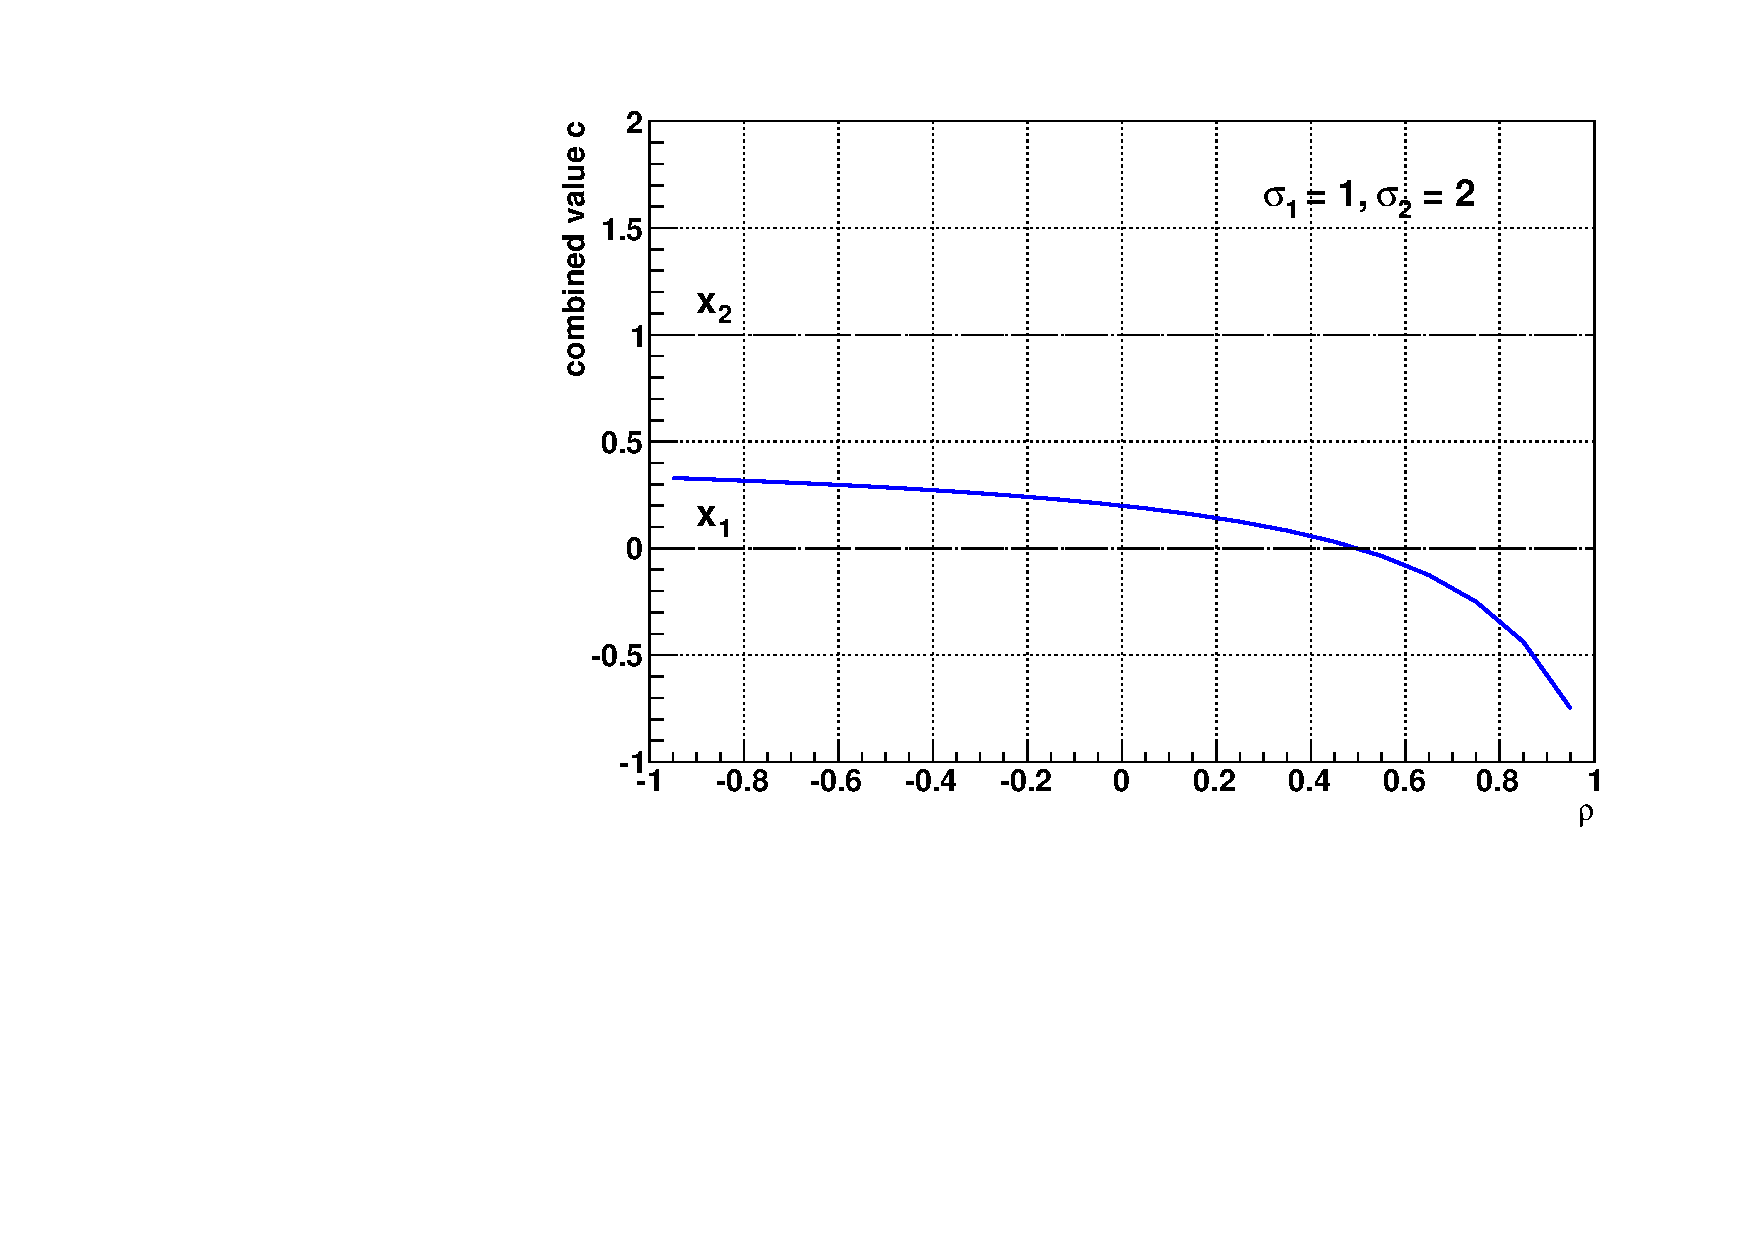
\includegraphics[width=0.48\textwidth]{c1.pdf}
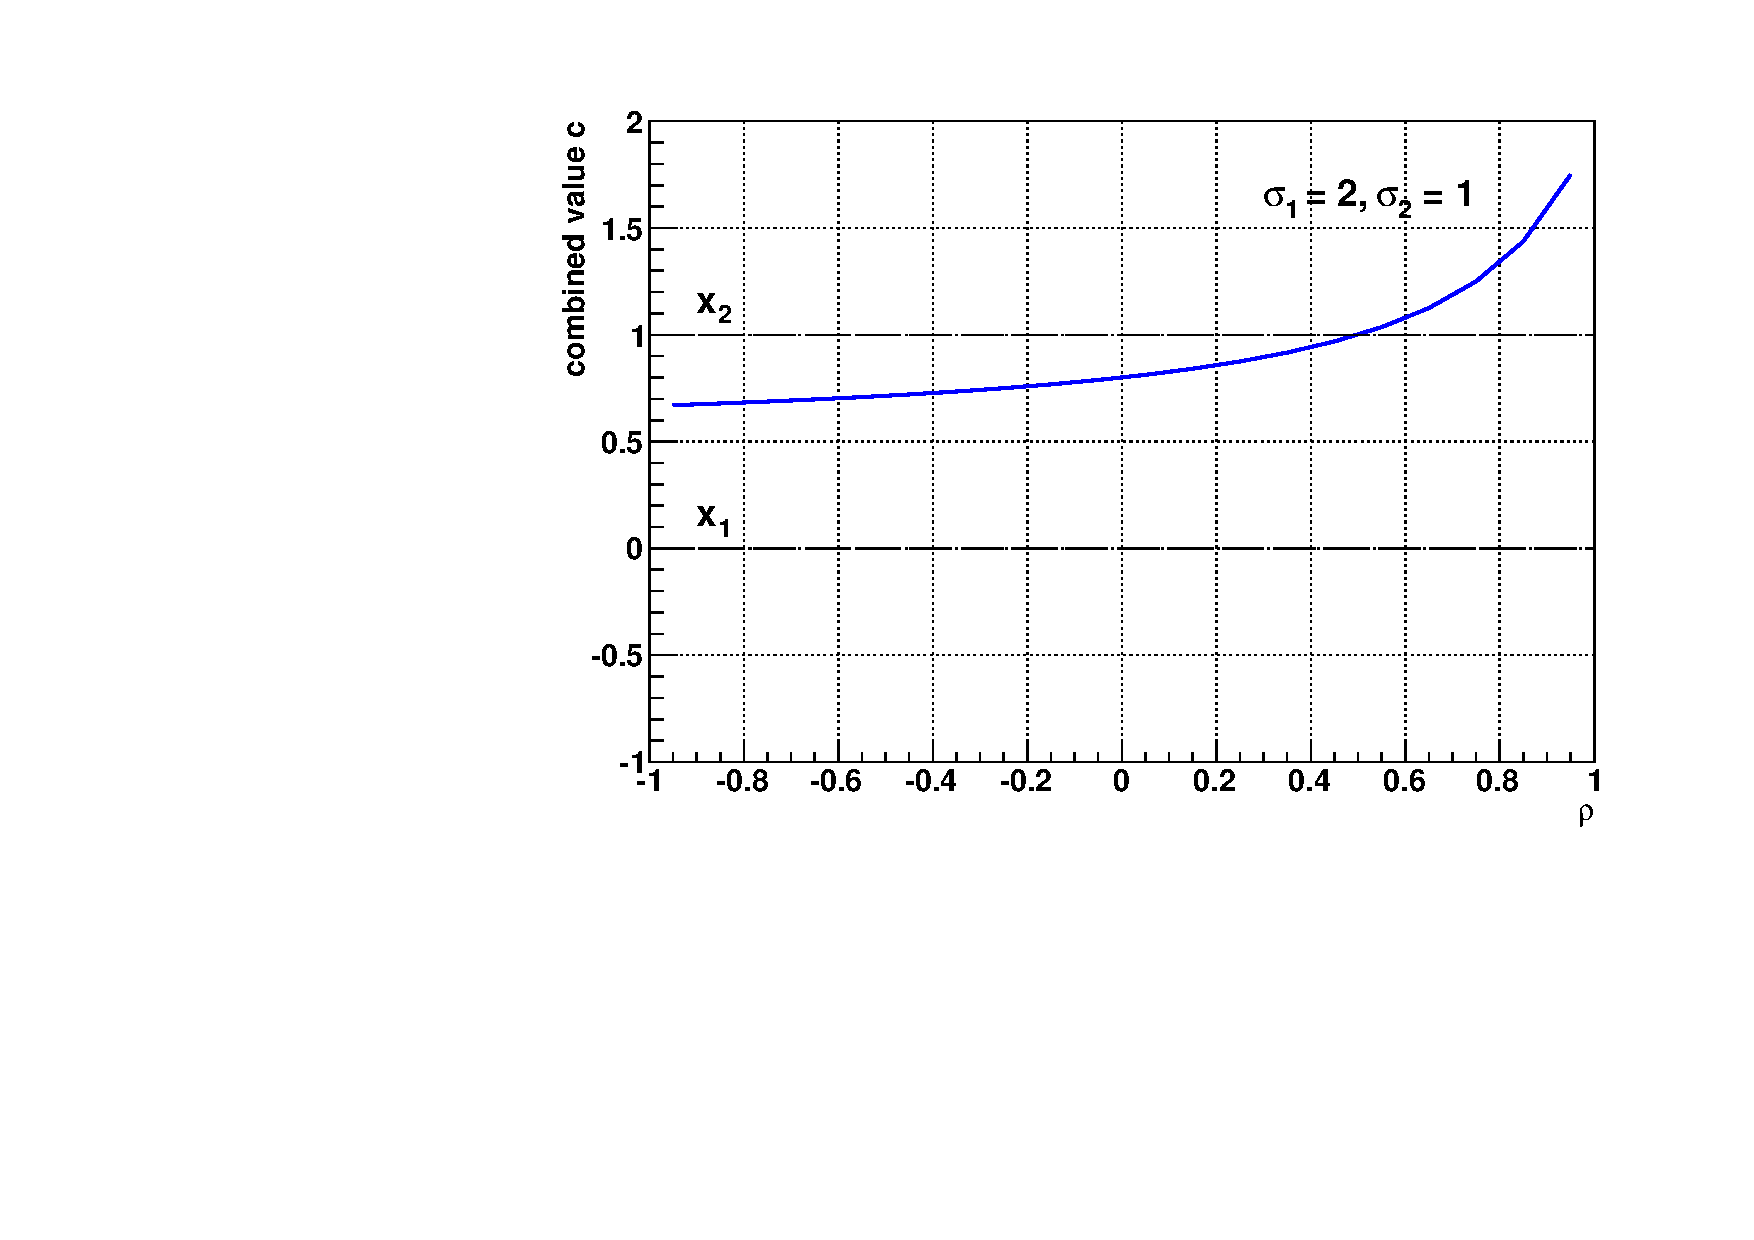
\includegraphics[width=0.48\textwidth]{c2.pdf}
\caption[.]{\label{fig:c1c2}
Least-squares solution $c$ as a function of the correlation coefficient~$\rho$.
Naively one expects the solution to fall between the two input values (indicated
by the long-dash lines), but when $\rho$ is large enough the solution lies outside that range.}
\end{center}
\end{figure}
%----------------------------------------------------------------



%----------------------------------------------------------------
\begin{figure}
\begin{center}
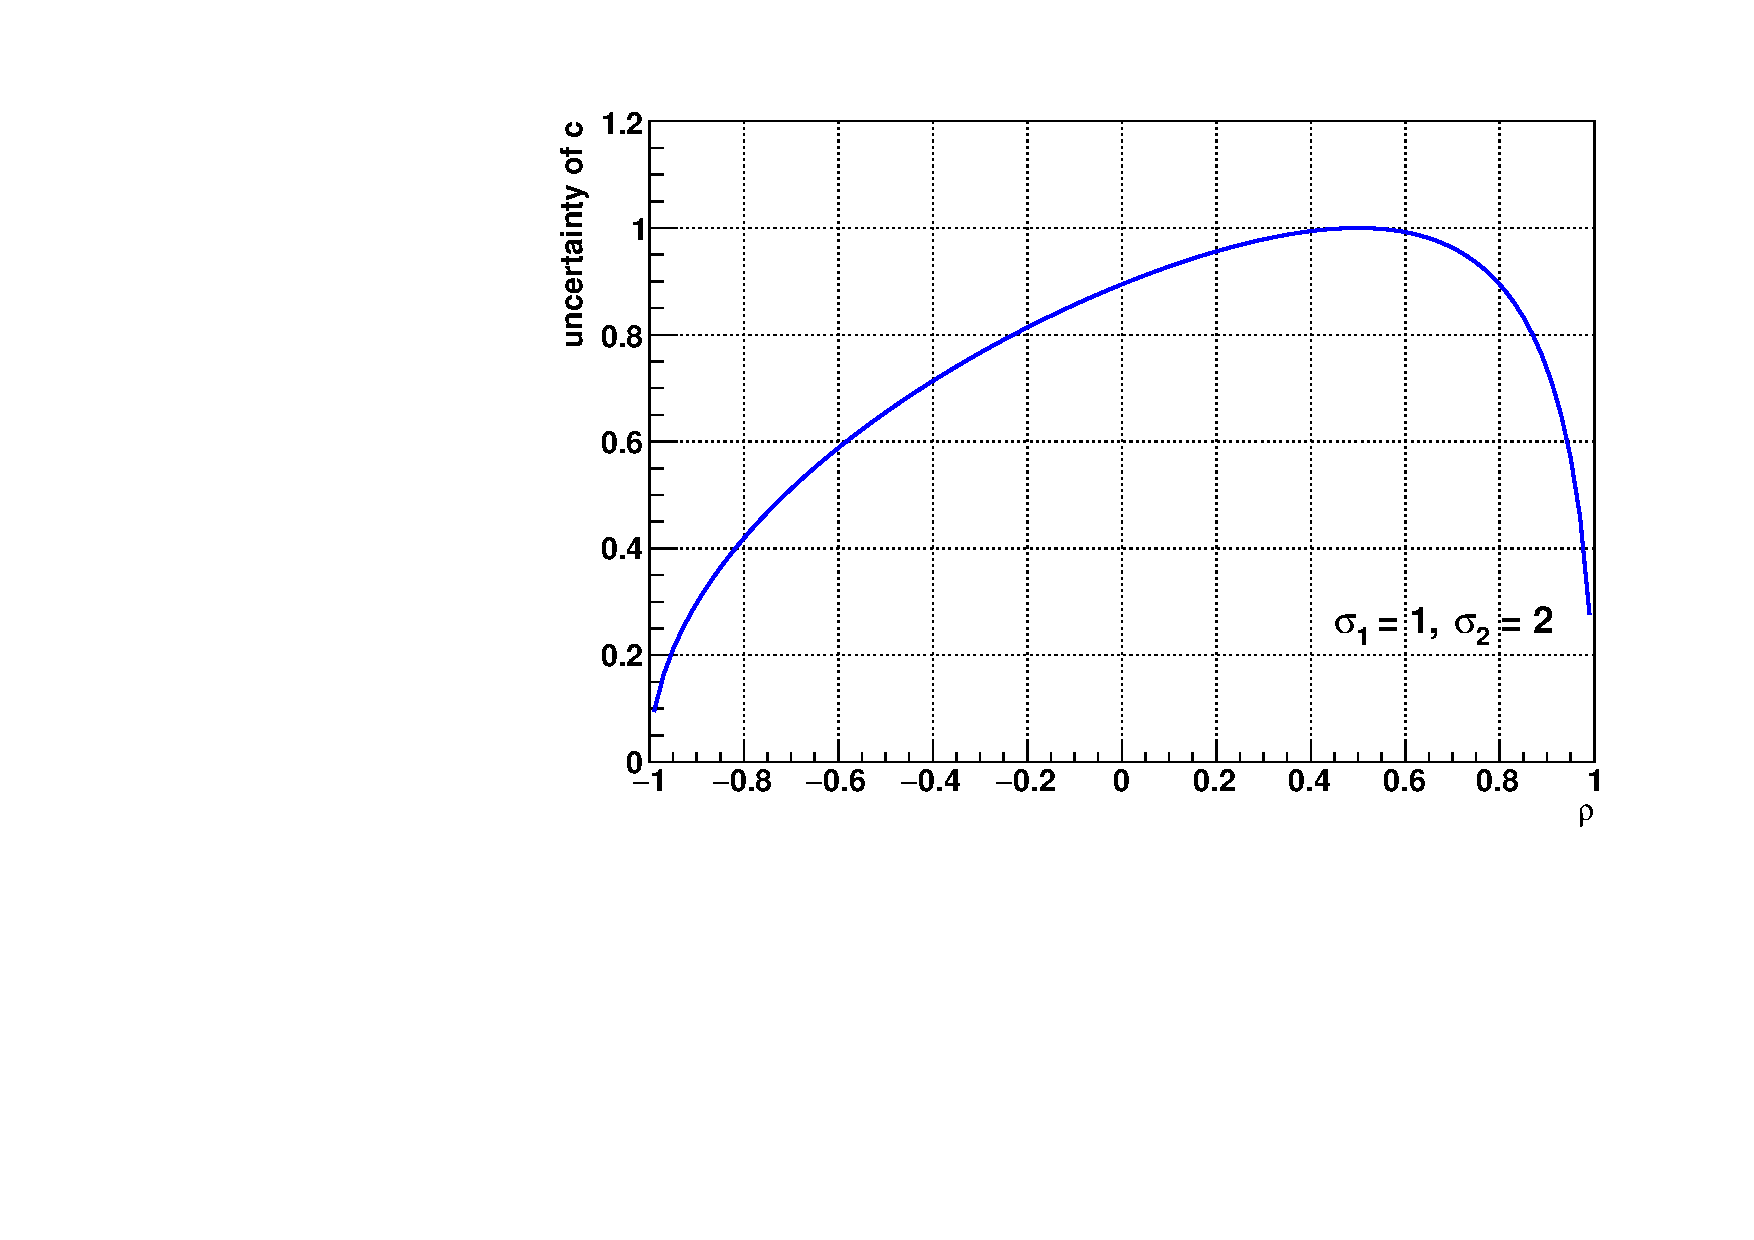
\includegraphics[width=0.48\textwidth]{cu.pdf}
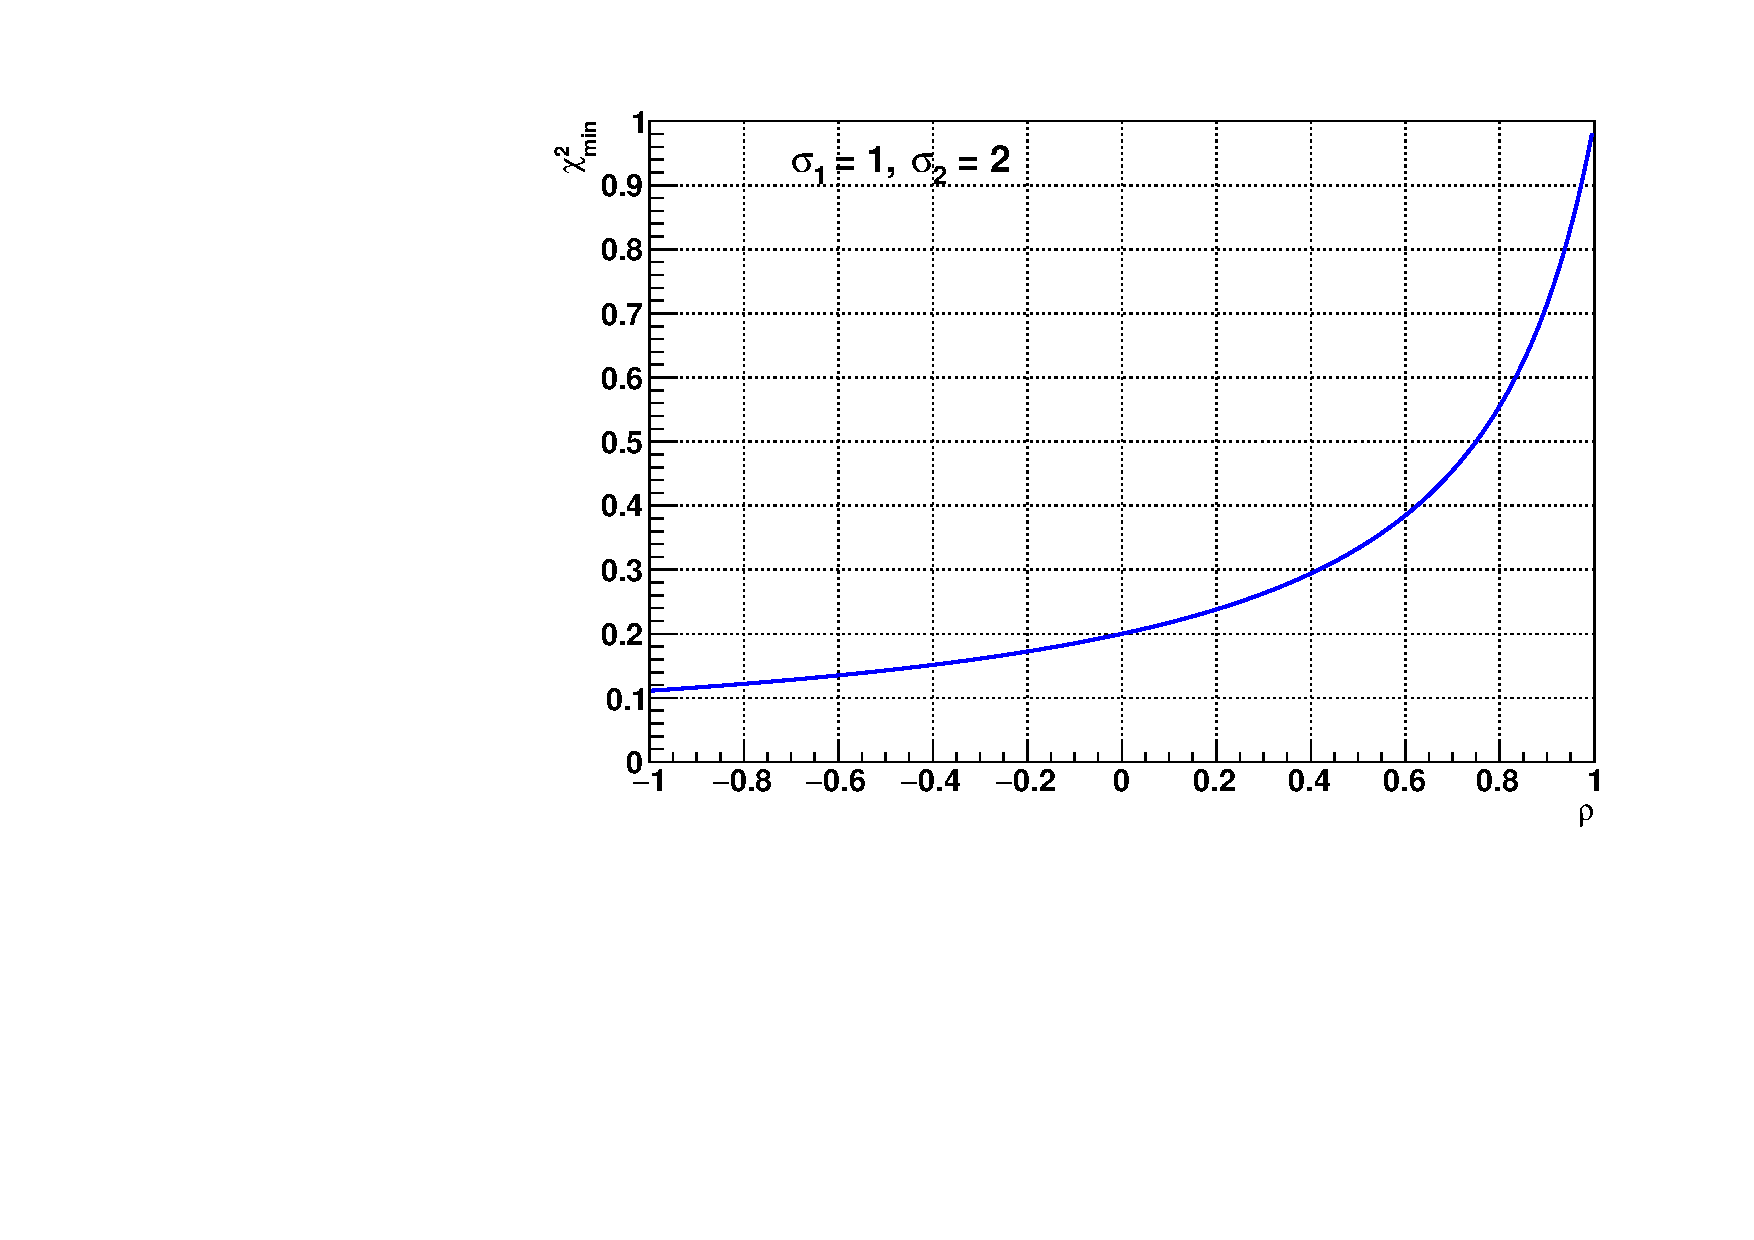
\includegraphics[width=0.48\textwidth]{cchisq.pdf}
\caption[.]{\label{fig:cucchisq}
Variation of the uncertainty $\uc$ (left) and $\chisqmin$ (right)
as a function of~$\rho$.  The numerical values are the same as
in Fig.~\ref{fig:c1c2}.}
\end{center}
\end{figure}
%----------------------------------------------------------------



\section{Analysis}
\par
The anomalies occur when $\rho$ is large and positive.  In the limit $\rho \rightarrow 1$,
one expects $\xb = \xa$, so any difference $\Delta = \xb - \xa \ne 0$ violates the expectations
about $\xb$ and $\xa$.   
\par
In order to gain some insight into this problem, 
we generalize the formulation of~$\chi^2$ to two independent parameters,
$\ca$ and $\cb$, in place of the single parameter $c$:  
\begin{equation} \label{eq:chisqdef2}
 \chi^2(\ca,\cb) =
 \left( \begin{array}{cc} \ca-\xa & \cb-\xb \cr \end{array} \right)
  \left( \begin{array}{cc}
   \uaq & \rho\ua\ub \cr \rho\ua\ub & \ubq \cr
          \end{array} \right)^{-1}
 \left( \begin{array}{c} \ca - \xa \cr \cb - \xb \end{array} \right) .
\end{equation}
If $\rho = 0$ then the solution is obvious: $\ca = \xa$ and $\cb = \xb$.
When $\rho \ne 0$, the solution is the same. % also $\ca = \xa$ and $\cb = \xb$.
\par
Figure~\ref{fig:chisq2D} shows contours of $\chi^2$ in the $(\ca,\cb)$ plane,
for $\rho = 0.1$, which results in a ``normal'' solution, and
$\rho = 0.9$, which results in an ``anomalous'' solution.
(We still have $\xa = 0$, $\xb = 1$, $\ua = 1$, and $\ub = 2\ua$.)
The thin diagonal line shows the constraint $\ca = \cb$ and the
thickened part of the diagonal line shows the intuitive expectation
$\xa < c < \xb$.
The dot shows the position of the minimum of~$\chi^2$ and 
the star shows the solution Eq.~(\ref{eq:csol}) obtained with the
constraint $\ca = \cb$.   For the case $\rho = 0.1$ the star falls
in the thick part of the diagonal line, while for $\rho =  0.9$ it
lies outside.

%----------------------------------------------------------------
\begin{figure}[hb]
\begin{center}
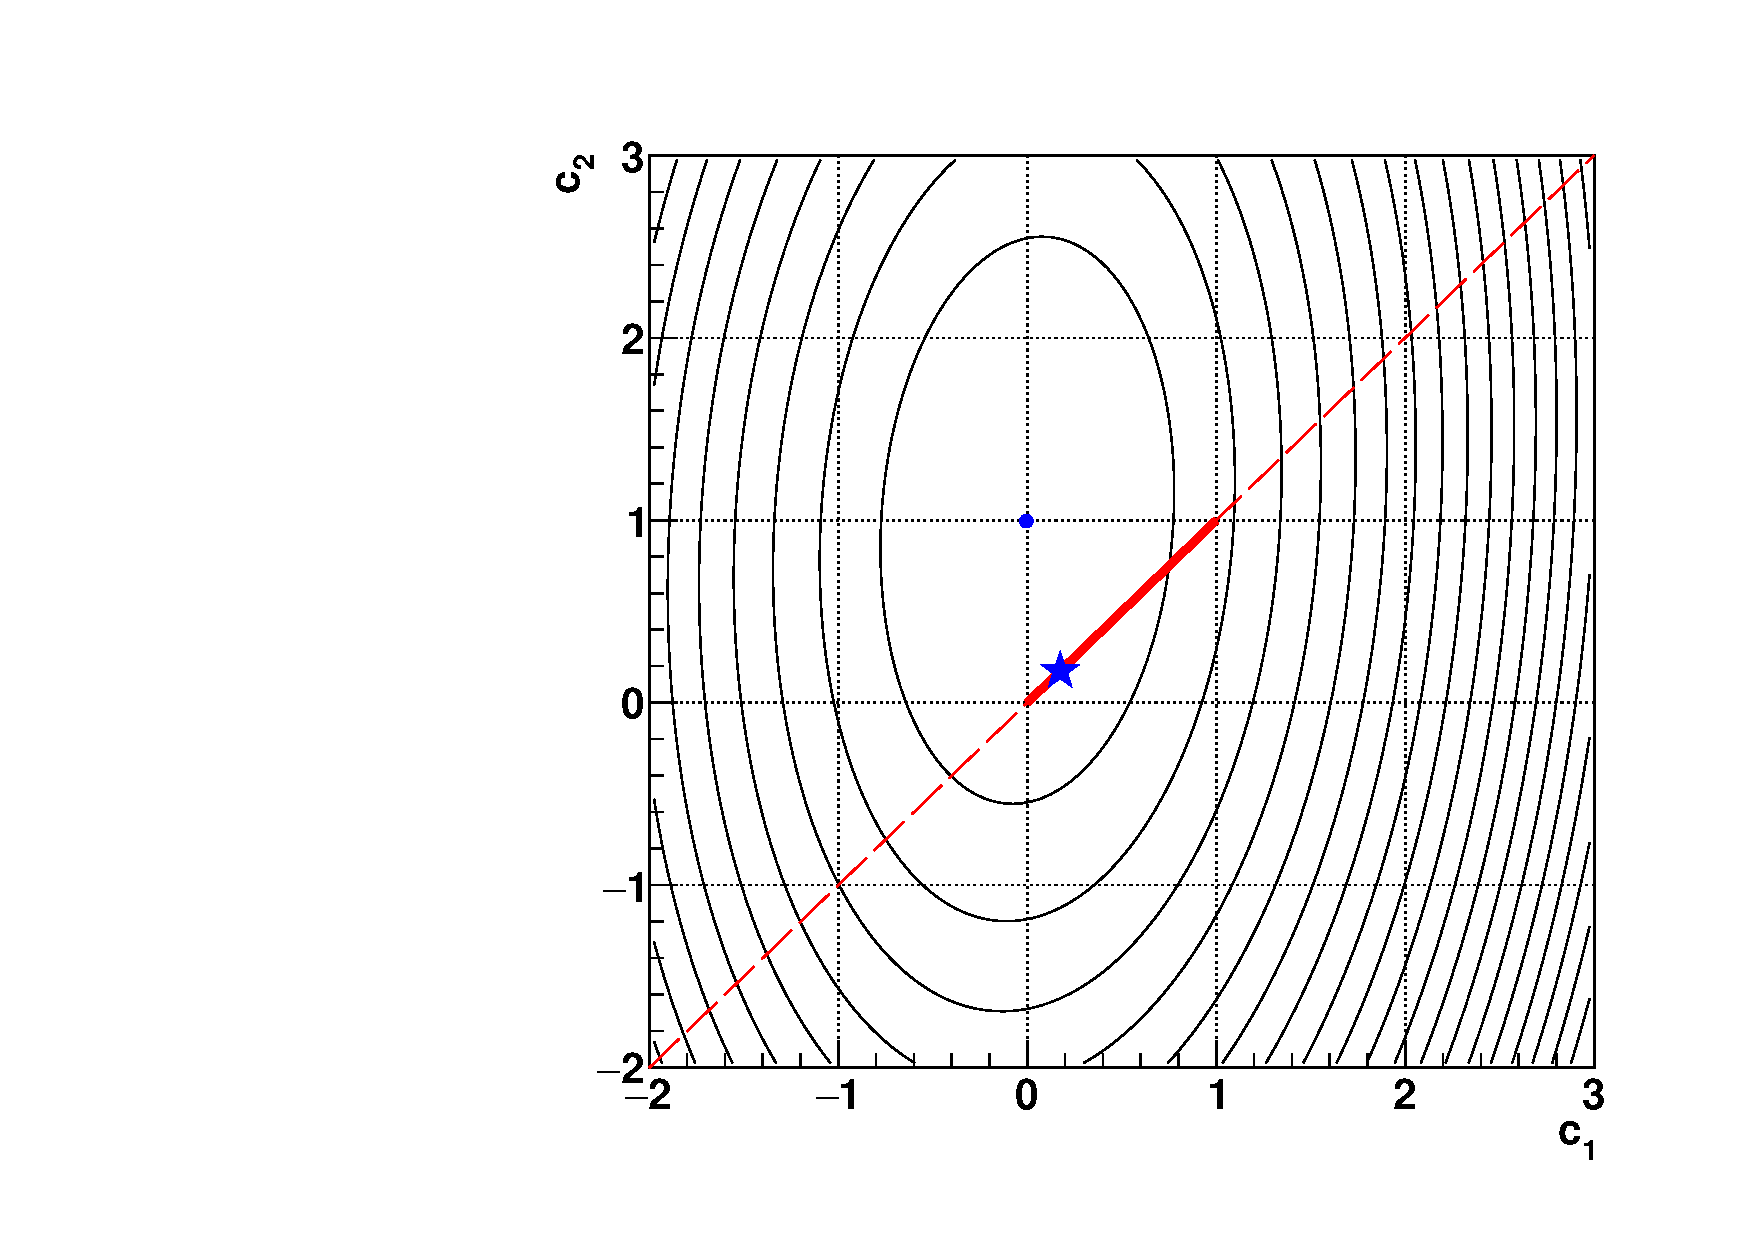
\includegraphics[width=0.48\textwidth]{contours_0p1.pdf}
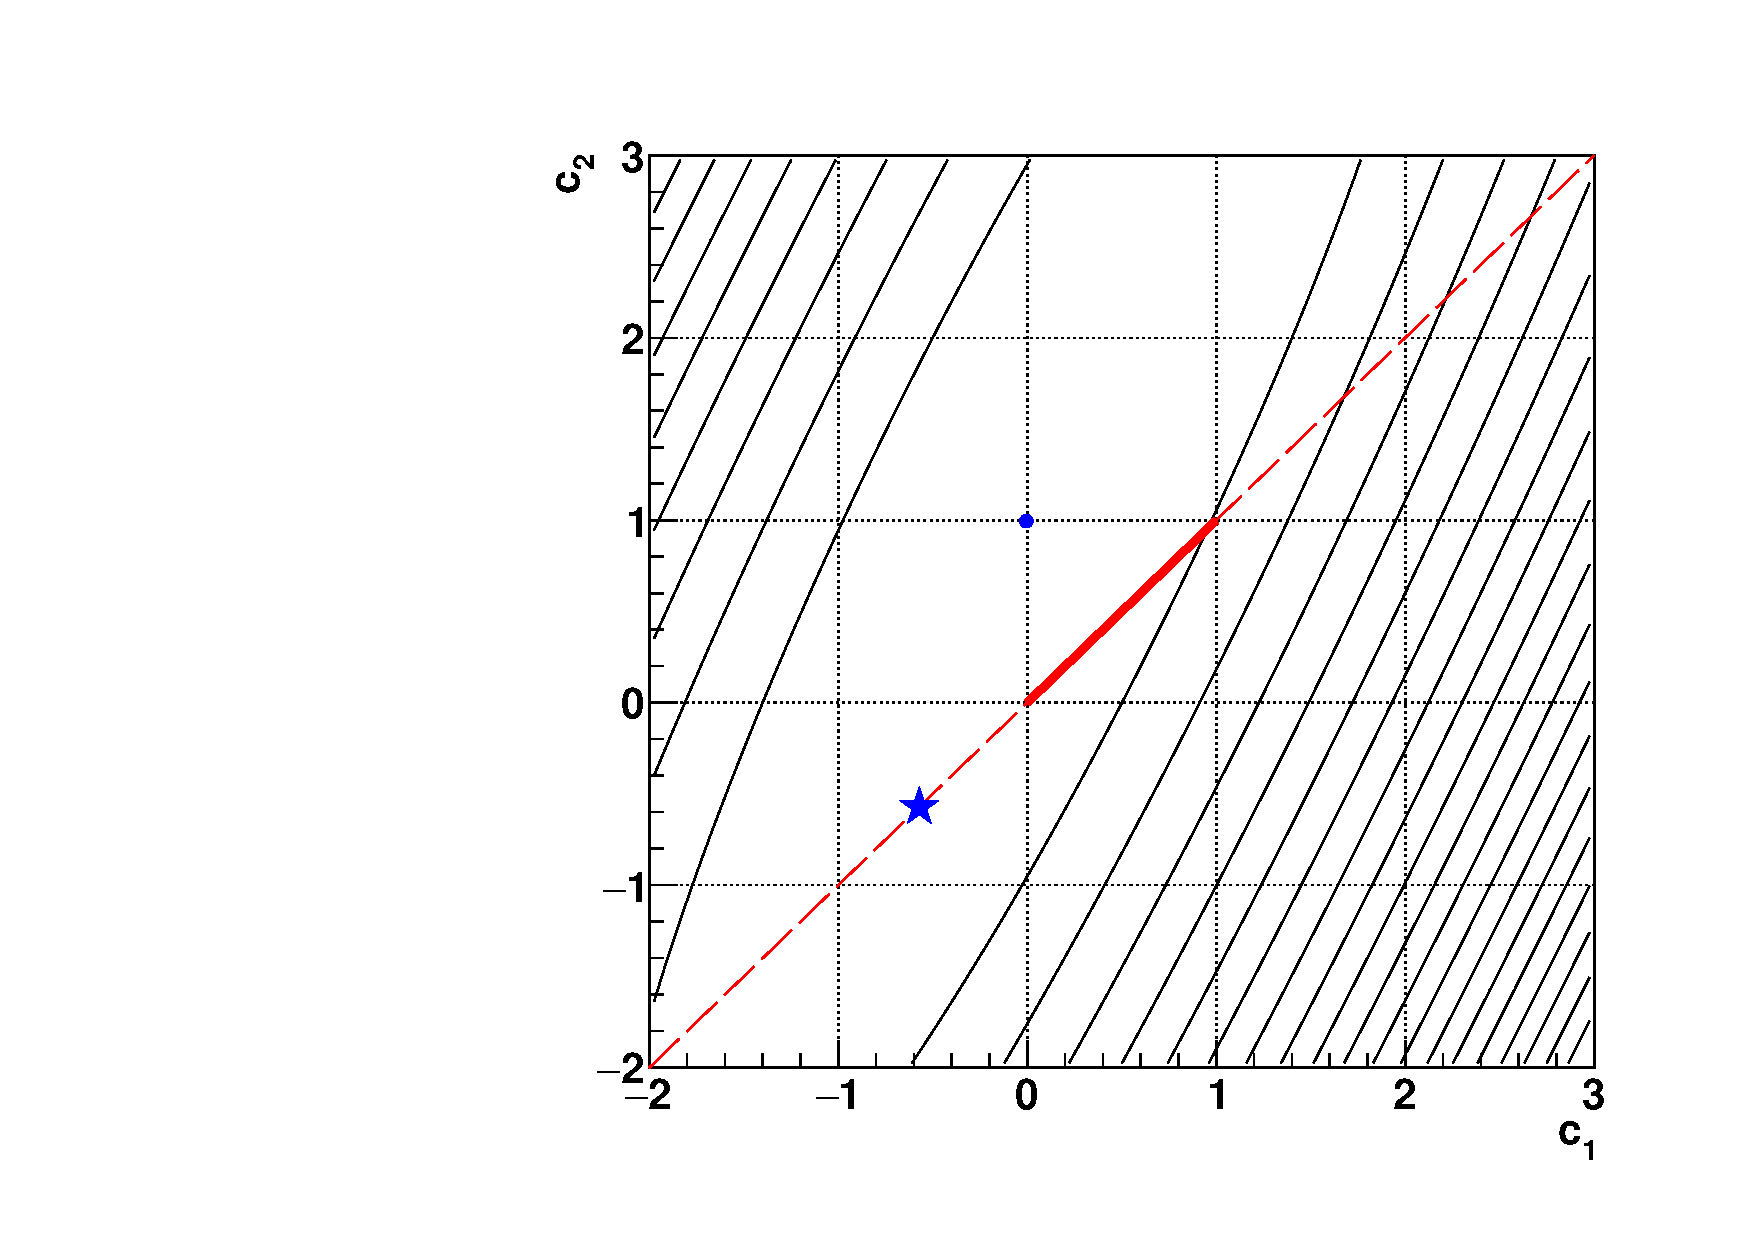
\includegraphics[width=0.48\textwidth]{contours_0p9.pdf}
\caption[.]{\label{fig:chisq2D}
Contours of $\chi^2$ in the $(\ca,\cb)$ plane.
The thin dashed diagonal line represents the case $\ca = \cb$,
with the solid thick part demarcating the expected range
$\xa < c < \xb$.  The blue dot shows the minimum of
$\chi^2$ and the star shows the solution Eq.~(\ref{eq:csol})
subject to the constraint $\ca = \cb$.}
\end{center}
\end{figure}
%----------------------------------------------------------------


%  ******************* SUPPRESS **********************
\iffalse
\par
The interpretation of $\chi^2$ as in Eq.~(\ref{eq:chisqdef}) is simple if
the inverse covariance matrix $\mathbf{V}^{-1}$ is diagonal.
We introduce a unitary transformation that relates $\mathbf{V}^{-1}$
to a diagonal matrix $\mathbf{W}^{-1}$.   This unitary transformation
will give us a linear combination of $\ca$ and $\cb$, and also of
the measurements $\xa$ and $\xb$, that are straight forward to handle.
This transformation will correspond to a rotation in the $(\ca,\cb)$ plane
such that the ellipses in Fig.~\ref{fig:chisq2D} are horizontal (or vertical).
\par
Proceeding with the calculation,
$$
 {\mathbf{V}}^{-1} = {\mathbf{R}}^{-1} \, {\mathbf{W}}^{-1} \, {\mathbf{R}} .
$$
We know ${\mathbf{V}}^{-1}$ and we know the off-diagonal elements of
${\mathbf{W}}^{-1}$ are zero.
\fi
%  ****************************************************


\section{Remedy}
\par
It is not clear that a remedy is needed.   As Lyons et~al. point out, if
$\xb$ is highly correlated with $\xa$, then if $\xa$ fluctuates above
the true value $\xtrue$, then so will $\xb$.   Consequently, one should
take $\xa$ and $\xb$ to perform an {\em extrapolation} rather than an
{\em interpolation}, which is precisely what this method provides
(see alo Fig.~\ref{fig:chisq2D}).
\par
Reference~\cite{Lyons} was concerned primarily with statistical correlations,
however.  Correlations caused by common systematic uncertainties are
fundamentally different -- see the earlier discussion on additive versus
multiplicative systematic uncertainties.  
{\bf MORE}



\newpage
\section{MORE WORK TO DO}
\par
Things I should still investigate:
\begin{enumerate}
\item
Point out that correlations between measurements of the same quantity
are what we examine here.   Correlations between measurements of
different quantities are also important but do not tend to display
the anomalous behavior described here.   (See Valassi.)
\item
Plot the distribution of $\chi^2$.
\item
Show that the variance of $c$ is minimized and is smaller
than taking the straight average.
\item
Point out that the exact values of the correlations are important
and that one should check the sensitivity of the central value
and its uncertainty under mild variations of the correlation coefficients.
\item
Despite the fact that $c$ is unbiased, it is still unreasonable to have
$c$ outside the range $[\xa,\xb]$ for the sake of a luminosity uncertainty.
Can we enforce $c = (\xa+\xb)/2$ as far as luminosity and similar uncertainties
are concerned?   What is the impact on the {\sl bias} and on the {\sl variance}?
\par
This is obvious.   The results above show that $c$ is pushed outside the
interval $[\xa,\xb]$ in the direction of whichever measurements has the
smaller uncertainty.   As far as luminosity is concerned, however, the
uncertainty on either of the measurements is irrelevant and there is no
reason to suppose that $c < \xa$ is better than $c > \xb$, or vice-versa.
\par
So...  it is important to check whether one of the experiments gives
better information about a nuisance parameter such as luminosity 
than the other experiment.
\par
This suggests that uncertainties on measured quantities and on nuisance
parameters {\sl somehow} need to be separated.
\item
Bring out the connection between the compatibility of measurement values
$\xa$ and $\xb$ as reflected in their difference $\xb - \xa$.
\item
What happens if a systematic uncertainty is {\bf not} Gaussian distributed?
Do a simulation with the luminosity distributed Gaussian, triangle, and box.
Perhaps consider other models for the pdf (thinking of theoretical uncertainties for example).
\item
Investigate Jens Erler's method.
\item
Improve the discussion of additive versus multiplicative uncertainties.
\item
What would be a Bayesian approach to this problem?
What is the posterior for $c$?   What happens if we enforce
$x_1 < c < x_2$ using the prior?
\item
Is there a way to couch this problem in the language of risk or cost analysis?
\item
Find a way to connect the bias (e.g. from taking the arithematic mean)
and the variance -- discuss the MSE in this problem.
\item
How would (Shannon) entropy enter this problem?
\item
Is there a way to apply machine learning to this problem?
One could train the algorithm (e.g. ANN) easily and then
apply it to the data.  Pay attention to bias.
The training should differentiate between random measurement
errors and correlated systematic errors/uncertainties.

\end{enumerate}





\begin{thebibliography}{9}

\bibitem{Lyons}
  L.~Lyons, D.~Gibaut and P.~Clifford,
  ``How to Combine Correlated Estimates of a Single Physical Quantity,''
  Nucl.\ Instrum.\ Meth.\ A {\bf 270}, 110 (1988).
  doi:10.1016/0168-9002(88)90018-6


\bibitem{Valassi} 
  A.~Valassi,
  ``Combining correlated measurements of several different physical quantities,''
  Nucl.\ Instrum.\ Meth.\ A {\bf 500}, 391 (2003).
  doi:10.1016/S0168-9002(03)00329-2

\bibitem{Nisius} 
  R.~Nisius,
  ``On the combination of correlated estimates of a physics observable,''
  Eur.\ Phys.\ J.\ C {\bf 74}, no. 8, 3004 (2014)
  doi:10.1140/epjc/s10052-014-3004-2


\bibitem{Erler} 
  J.~Erler,
  ``On the Combination Procedure of Correlated Errors,''
  Eur.\ Phys.\ J.\ C {\bf 75}, no. 9, 453 (2015)
  doi:10.1140/epjc/s10052-015-3688-y




\end{thebibliography}


\end{document}
